\chapter{Introducción específica} % Main chapter title

\label{Chapter2}

%----------------------------------------------------------------------------------------
%	SECTION 1
%----------------------------------------------------------------------------------------
En este capítulo se profundiza en aquellos aspectos clave para el desarrollo de este trabajo.
En primer lugar, se presentan los requerimientos de sistema y se amplía la información acerca de los modelos de 
inteligencia artificial que se han utilizado.
Finalmente, se expone el conjunto de técnicas y herramientas que se han aplicado a dichos modelos.

\section{Requerimientos del sistema}
Para llevar a cabo este trabajo
se identificaron una serie de requerimientos fundamentales.
A continuación se listan aquellos que están directamente relacionados con la implementación:

\begin{enumerate}
	\item Requerimientos del servidor:
	      \begin{enumerate}
		      \item El servidor debe alojar y administrar la información relativa al \textit{dataset} y la configuración del modelo LLM.
		      \item El servidor debe contar con los \textit{prompts} necesarios para especializar la respuesta de  la inteligencia artificial.
		      \item Al ser desplegado, el servidor deberá acceder al módulo LLM y utilizarlo en el procesamiento de peticiones entrantes.
		      \item El servidor debe dar acceso a clientes externos a través del protocolo API REST.
		      \item Los servicios REST deben aceptar entrada de texto en varios formatos: pdf, txt, docx o texto plano en el cuerpo de la petición.
		      \item Los servicios REST devolverán la respuesta en formato simple HTML para su cómoda visualización en un navegador.
		      \item El prototipo del servidor debe de tener una disponibilidad del 100\% durante la demostración.
	      \end{enumerate}
	\item Requerimientos del módulo LLM:
	      \begin{enumerate}
		      \item El módulo LLM debe aceptar entrada de texto y generar texto como salida.
		      \item En caso de que el texto de entrada sea legible, el módulo LLM debe aportar una respuesta con un detalle y profundidad razonables,
		            además de ser coherente con las instrucciones recibidas.
		      \item El módulo se ajustará a los \textit{prompts} recibidos para que, con el mismo contexto,
			  		devuelva información enfocada en un aspecto específico de la narrativa.
		      \item El tiempo de respuesta del módulo LLM debe estar en un rango de tiempo razonable para un servicio REST (no más de 5 minutos).
	      \end{enumerate}
\end{enumerate}

%----------------------------------------------------------------------------------------
%	SECTION 2
%----------------------------------------------------------------------------------------

\section{Modelos extensos de lenguaje}
Para abordar los requisitos de generación de texto resultó fundamental la utilización 
de modelos extensos de lenguaje, comúnmente denominados \textit{Large Language Models} (LLM).
Estos modelos son entrenados sobre enormes volúmenes de datos textuales para especializarlos
en predecir la secuencia de texto más probable dada una entrada previa.
Esta habilidad les permite generar texto de forma coherente con el contexto
al adaptarse al tono, estilo y contenido esperado.

Los LLM se basan en redes neuronales profundas que manejan miles de millones de parámetros
(lo que justifica su clasificación como modelos ``extensos'') para identificar patrones complejos del lenguaje natural \cite{att_is_all_you_need}. 
Estos modelos utilizan \textit{tokens} como unidad básica de texto en su procesamiento.
Los \textit{tokens} pueden representar palabras completas, fragmentos de palabras o signos de puntuación,
dependiendo del sistema de tokenización utilizado.
Estos \textit{tokens} se convierten posteriormente en vectores numéricos
mediante una capa de \textit{embedding} \cite{mikolov2013efficient}, que permite al modelo operar sobre ellos.

Los LLM modernos utilizan la arquitectura de \textit{transformers} \cite{att_is_all_you_need},
un tipo de red neuronal que permite procesar secuencias de texto en paralelo y asignar diferentes niveles de relevancia
(atención) a distintas partes del texto mediante un mecanismo llamado \textit{self-attention} \cite{att_is_all_you_need}.
Esta arquitectura supera notablemente a estructuras anteriores como \textit{Long-Short Term Memory} \cite{hochreiter1997long}
o \textit{Gated Recurrent Unit} \cite{cho2014learning} en cuestiones de eficiencia y rendimiento.

Además de su capacidad de paralelización y memoria a largo plazo, los LLM basados en \textit{transformers} operan 
mediante la predicción de la siguiente cadena de \textit{tokens} a partir del contexto previo.
En este proceso hay elementos que controlan la generación, entre los que se destaca la temperatura \cite{radford2019language}.
La temperatura regula la aleatoriedad de los \textit{tokens}: valores bajos tienden a generar respuestas deterministas,
mientras que valores altos proporcionan respuestas más diversas y creativas\footnote{
	Esto también aumenta las probabilidades de que esta respuesta sea incoherente, también llamada alucinación.
}. Existen otros parámetros que controlan la variedad del texto, por ejemplo \textit{top-k} y \textit{top-p} \cite{holtzman2019curious}.

A medida que los LLM aumentan en extensión de parámetros y profundidad de entrenamiento, empiezan a manifestar cualidades
que no fueron explícitamente programadas. Entre estas capacidades destacan el razonamiento en múltiples pasos,
traducción automática entre idiomas, capacidad de responder a preguntas complejas y generación creativa y coherente de texto
que va más allá de la simple predicción de cadenas de texto.

Por ejemplo, modelos como GPT-3 \cite{Brown2020GPT3} de OpenAI, PaLM \cite{chowdhery2022palm} de Google 
y LLaMA \cite{touvron2023llama} de Meta han demostrado un rendimiento notable
en multitud de tareas complejas como realizar inferencias lógicas, resolver problemas matemáticos,
resumir textos extensos y generar código a partir de descripciones en lenguaje natural.
Esto no solo amplía el espectro de aplicaciones prácticas de los LLM,
sino que también plantea nuevas líneas de investigación para comprender cómo el tamaño y
la calidad del entrenamiento impactan en la adquisición de habilidades cognitivas sofisticadas.

%----------------------------------------------------------------------------------------
%	SECTION 3
%----------------------------------------------------------------------------------------

\section{Ingeniería de \textit{prompts}}
La ingeniería de \textit{prompts} (\textit{prompt engineering}) es una técnica fundamental en la optimización de la salida de los modelos extensos de lenguaje
que se basa en guiar el proceso de razonamiento del modelo hacia un objetivo específico a través de un conjunto de entradas textuales.
A diferencia de la programación tradicional, que se expresa de forma explícita la lógica mediante el uso de código en un lenguaje de programación,
el comportamiento de los LLM se guía mediante lenguaje natural.

Esta técnica ha emergido como una nueva disciplina en la que intervienen conceptos linguísticos y computacionales.
La forma en la que se redacta una instrucción puede influir de forma notable en la coherencia, relevancia, creatividad
y precisión de las respuestas.

Entre las estrategias comunes de ingeniería de prompts se encuentran \textit{zero/few-shot prompting} \cite{brown2020language}\cite{kojima2022large},
que emplea ejemplos en el \textit{prompt} para guiar la generación; \textit{chain of thought prompting} \cite{wei2022chain} invita al modelo a razonar explícitamente
los pasos intermedios antes de llegar a la conclusión; o \textit{prompt chaining} \cite{promptchaining2023} que invita al modelo a realizar un análisis previo
sobre el contexto o instrucciones para enfocar la salida.
En la figura \ref{fig:prompting} se ilustra cómo estas estrategias de instrucción afectan directamente la salida generada por el modelo.
Cabe destacar que las distintas técnicas de \textit{prompting} descritas no son excluyentes entre sí,
sino que pueden combinarse de manera complementaria, lo que potencia la capacidad de razonamiento
y la precisión de los LLM en tareas complejas.
% \footnote{
% 	Imagen obtenida del material del curso de especializacion en inteligencia artificial de la FIUBA,
% 	materia de \textit{LLM} \cite{fiubaPrompt} 
% 	}
\begin{figure}[htbp]
	\centering
	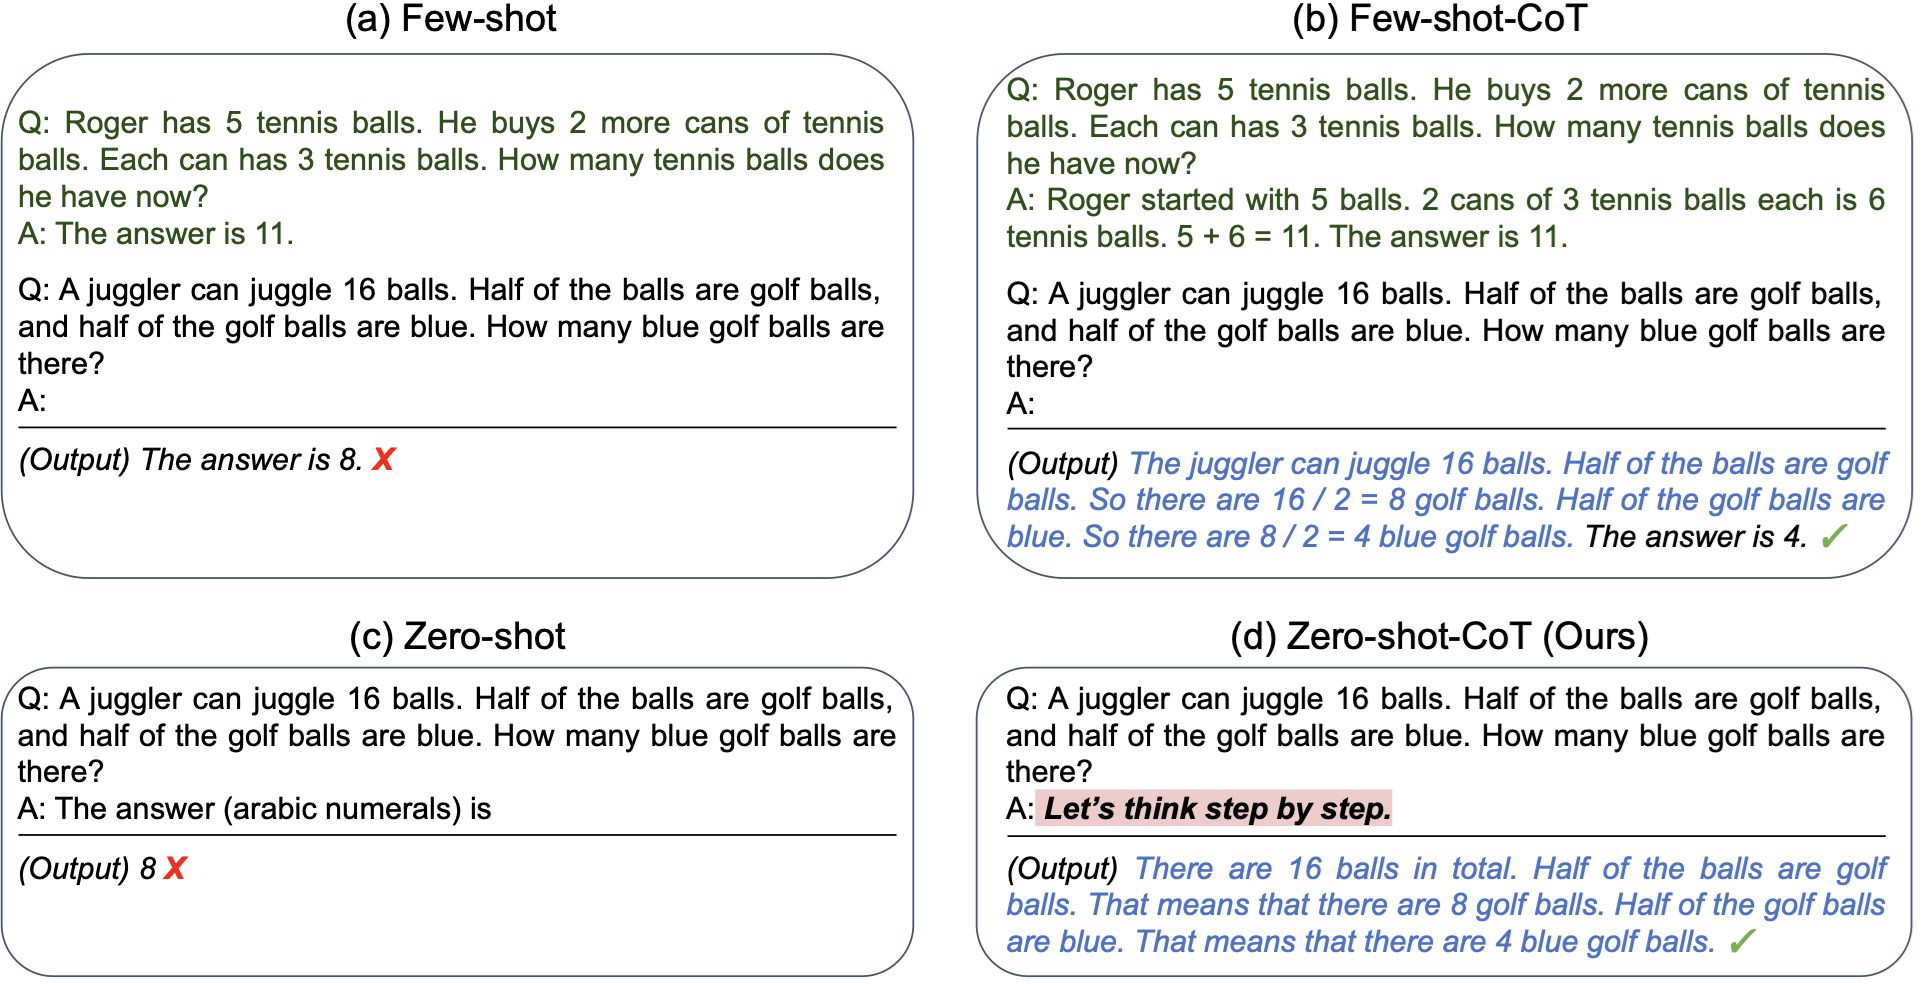
\includegraphics[width=0.9\textwidth]{./Figures/prompting.png}
	\caption{Ejemplo de uso de técnicas de \textit{prompting}.}
	\label{fig:prompting}
\end{figure}

A su vez, la ingeniería de \textit{prompts} ha demostrado ser fundamental en aquellos contextos en los que
el \textit{fine-tuning} no es viable, ya que hay muchos modelos cerrados que solo son accesibles a través de una API
y la capacidad de modificar su comportamiento sin reentrenamiento se vuelve crucial.
Por lo tanto, esta técnica se convierte en una herramienta práctica, eficiente y cada vez más sofisticada
para adaptar modelos generalistas a tareas específicas.

%----------------------------------------------------------------------------------------
%	SECTION 4
%----------------------------------------------------------------------------------------

\section{Ajuste fino}
El ajuste fino (\textit{fine-tuning}) \cite{howard2018universal} es una técnica de entrenamiento de modelos extensos de lenguaje 
que permite adaptar un modelo previamente entrenado a una tarea en específico.
A diferencia del entrenamiento desde cero, esta técnica parte de una base
y lo especializa utilizando un conjunto mucho más pequeño y específico de datos.
De este modo se reduce significativamente el coste computacional a la vez que se aprovecha
la capacidad predictiva del modelo del que se parte.

Para llevar a cabo el ajuste fino, se conservan la estructura y los parámetros previamente entrenados del modelo base,
evitando así la necesidad de un entrenamiento completo desde cero.
En la práctica, el proceso de \textit{fine-tuning} suele centrarse en modificar únicamente una parte reducida del modelo,
como las capas superiores, que son las más cercanas a la salida y, por tanto,
más fácilmente adaptables a tareas específicas.
Alternativamente, pueden integrarse nuevas capas que se entrenan sin alterar el resto del modelo.
Esta aproximación permite preservar los conocimientos generales adquiridos durante el preentrenamiento
mientras se optimiza la capacidad del modelo para tareas concretas.

Además, en escenarios con recursos computacionales limitados
se utilizan técnicas de ajuste fino eficiente (parameter-efficient fine-tuning, PEFT),
como LoRA (\textit{Low-Rank Adaptation}) \cite{hu2021lora},
\textit{prefix tuning} \cite{li2021prefix} o \textit{prompt tuning}.
Estas estrategias reducen la cantidad de parámetros que deben entrenarse,
lo que no solo disminuye el tiempo de ajuste y el consumo de memoria,
sino que también facilita la reutilización del modelo base en múltiples contextos sin interferencia entre tareas.

Al adaptar un modelo generalista a contextos específicos,
se logra una mejora sustancial en la precisión, relevancia y
sensibilidad del modelo frente a matices del lenguaje propios del área de aplicación.
No obstante, es fundamental contar con datos de alta calidad y
bien etiquetados para evitar la sobreespecialización o la introducción de sesgos.

\pagebreak
%----------------------------------------------------------------------------------------
%	SECTION 5
%----------------------------------------------------------------------------------------
\section{LM Studio y otras tecnologías}
LM Studio \cite{lmstudio} es una plataforma de código abierto diseñada para facilitar la interacción
y despliegue de modelos extensos de lenguaje (LLM) de manera local,
lo que permite a los usuarios ejecutar y experimentar con modelos sin depender de servicios en la nube.
Esta herramienta destaca por su integración sencilla, soporte para múltiples formatos de modelos y una interfaz amigable.

Una de las ventajas clave de LM Studio es su capacidad para manejar modelos grandes y complejos con eficiencia.
Ofrece funcionalidades como la gestión de memoria optimizada,
soporte para cuantización y carga progresiva de modelos
lo que permite que usuarios con recursos limitados puedan aprovechar la potencia de los LLM
sin necesidad de infraestructura costosa.
Además, LM Studio facilita la personalización de modelos mediante interfaces accesibles,
lo que la convierte en una opción popular tanto para investigadores como para desarrolladores
que desean incorporar inteligencia artificial avanzada en sus proyectos.

Para la implementación del \textit{backend} de la aplicación que interactúa con LM Studio, se utilizó \textit{Python},
un lenguaje de programación ampliamente adoptado en el ámbito de la inteligencia artificial por su simplicidad
y la gran cantidad de bibliotecas disponibles.
Se empleó la biblioteca de FastAPI \cite{fastapi} en al construcción del servidor web gracias a su sintaxis intuitiva,
lo que facilitó la creación de \textit{endpoints} eficientes para la comunicación entre el usuario y el modelo.

Por otro lado, \textit{PyTorch} \cite{pytorch} es la biblioteca de referencia para el desarrollo 
y entrenamiento de modelos de aprendizaje profundo, incluyendo los LLM.
Proporciona una interfaz dinámica y flexible que permite tanto el entrenamiento
como la inferencia eficiente en hardware acelerado, y es compatible con múltiples plataformas.